J'ai d'abord créé tout dans un docker à l'aide de docker-compose.
Ceci était plus simple car comme ça cela créé tout en même temps et on n'a plus qu'a les initialiser
après

On a donc créé 3 types : Shard, Mongos et config Servers:

\begin{itemize}
    \item Le shard : Il contiendra donc une partie des données, chaque shard peuvent être déployé en
    tant que replica sets
    \item Mongos : Il va agir comme « routeur » il fournira donc une interface à chaque client de
    l'application
    \item Config servers : C'est là où on va enregistrer les configurations pour le cluster
\end{itemize}

On va donc d'abord créer 3 serveurs de sharding et ensuite créer donc ces replica sets.
Les avantages à ceux-ci sont nombreux :

\begin{itemize}
    \item \textbf{Haute disponibilité} : On assure donc la redondance des données pour la gestion du sharding. Si
    un des membres tombent en panne cela assure toujours la mise en place de ce sharding
    \item \textbf{Optimisation des ressources }: En configurant le sharding avant les replica sets, vous pouvez
    évaluer la charge de travail et les besoins de chaque shard individuellement avant de déployer
    des replica sets. Cela vous permet d'optimiser l'allocation des ressources en fonction des
    exigences spécifiques de chaque shard, plutôt que de provisionner des replica sets pour tous les
    shards dès le départ.
    \item \textbf{Flexibilité dans l'ajout de replica sets }: En configurant d'abord le sharding, vous pouvez ajouter
    des replica sets à chaque shard au fur et à mesure de vos besoins. Cela vous offre une plus
    grande flexibilité dans l'ajustement de la capacité de stockage et de traitement de chaque shard
    individuellement, en ajoutant des membres supplémentaires aux replica sets existants ou en
    créant de nouveaux replica sets si nécessaire.
    \item \textbf{Évolutivité}: Le sharding permet de répartir les données sur plusieurs shards, ce qui permet
    d'atteindre une capacité de stockage et une capacité de traitement beaucoup plus importantes.
    L'utilisation de replica sets avec sharding permet de répartir également la charge de travail sur
    les membres du replica set, offrant ainsi une meilleure évolutivité horizontale de l'ensemble du
    système.
    \item \textbf{Simplification de la configuration initiale }: En configurant d'abord le sharding, vous pouvez
    réduire la complexité de la configuration initiale, en vous concentrant d'abord sur la mise en
    place de la répartition des données sur plusieurs shards. Une fois que le sharding est en place et
    que vous avez évalué les performances, vous pouvez ensuite configurer les replica sets pour
    chaque shard individuellement.
\end{itemize}

\begin{figure}[H]
    \centering
    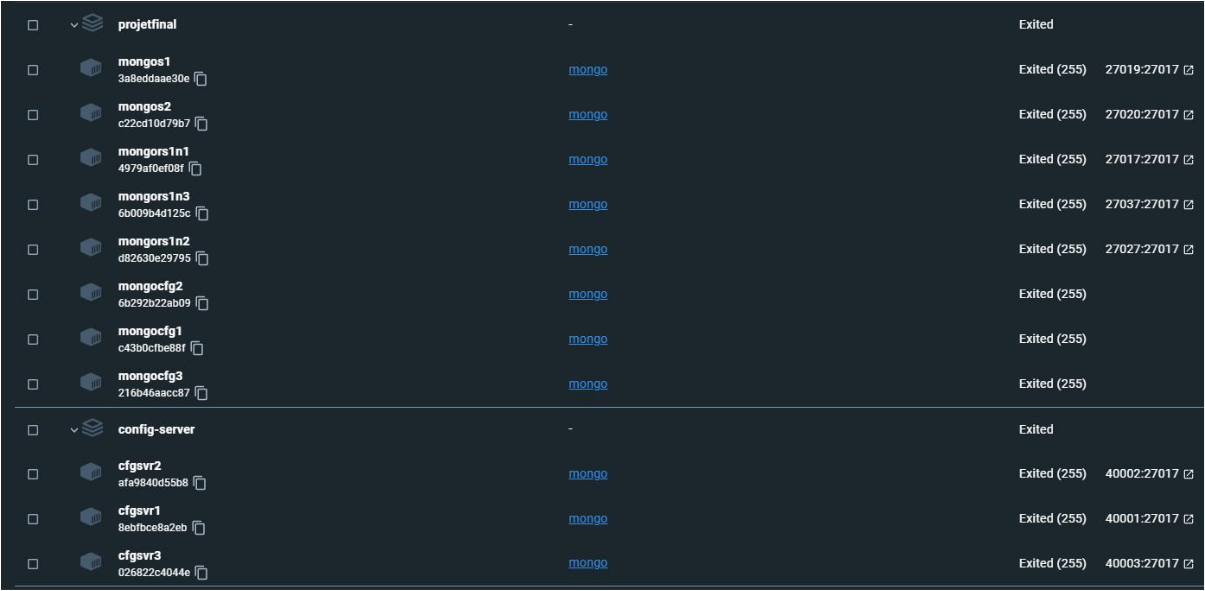
\includegraphics[width=\textwidth]{./img/alex.png}
    \caption{Instances des containeurs de MongoDB}
    \label{fig:alex-container-instance}
\end{figure}

On peut donc voir les différents type d'instance docker créé pour chacun des shardings, routeurs, config
servers.
Pour la partie mise en place, comment les bases de données sont utilisées, il faudra se référer à d'autres
parties qui vont expliquer comment ils ont utilisés ces données.
